\documentclass{article}
\usepackage[utf8]{inputenc}
\usepackage{listings}
\usepackage{multimedia} % to embed movies in the PDF file
\usepackage{graphicx}
\usepackage{comment}
\usepackage[english]{babel}
\usepackage{amsmath}
\usepackage{amsfonts}
\usepackage{wrapfig}
\usepackage{multirow}
\usepackage{verbatim}
\usepackage{float}
\usepackage{cancel}
\usepackage{caption}
\usepackage{subcaption}
\usepackage{/home/cade/Homework/latex-defs}
\usepackage{/home/cade/Homework/jlcode}


\title{AMATH 536 Problem Set 1}
\author{Cade Ballew \#2120804}
\date{April 15, 2022}

\begin{document}
	
\maketitle
	
\section{Problem 1}
\subsection{Part a}
Consider a birth-death process in which $\lambda=\mu$ which starts with $a>0$ individuals. Then, for $n\geq1$, and a small time-interval $\Delta t$,
\begin{align*}
p_n(t+\Delta t)=\lambda\Delta t(n-1)p_{n-1}(t)+(1-2\lambda n\Delta t)p_n(t)+\lambda\Delta t(n+1)p_{n+1}(t),
\end{align*}
so 
\begin{align*}
\frac{p_n(t+\Delta t)-p_n(t)}{\Delta t}&=\lambda(n-1)p_{n-1}(t)-2\lambda n p_n(t)+\lambda(n+1)p_{n+1}(t).
\end{align*}
Taking the limit of both sides,
\begin{align*}
\frac{d p_n(t)}{dt}=\lim_{\Delta t\to0}\frac{p_n(t+\Delta t)-p_n(t)}{\Delta t}&=\lambda(n-1)p_{n-1}(t)-2\lambda n p_n(t)+\lambda(n+1)p_{n+1}(t).
\end{align*}
For the $n=0$ case, 
\begin{align*}
	p_0(t+\Delta t)=1\cdot p_0(t)+\lambda\Delta t p_{1}(t),
\end{align*}
so 
\begin{align*}
	\frac{p_0(t+\Delta t)-p_0(t)}{\Delta t}=\lambda p_{1}(t).
\end{align*}
Taking the limit of both sides,
\begin{align*}
	\frac{d p_0(t)}{dt}=\lim_{\Delta t\to0}\frac{p_0(t+\Delta t)-p_0(t)}{\Delta t}=\lim_{\Delta t\to0}\lambda p_{1}(t)=\lambda p_{1}(t).
\end{align*}
Then, by definition,
\begin{align*}
\frac{\partial P(s,t)}{\partial t}&=\sum_{n=0}^\infty\frac{d p_n(t)}{d t}s^n=\lambda\sum_{n=2}^\infty(n-1)p_{n-1}(t)s^n-2\lambda\sum_{n=1}^\infty n p_n(t)s^n+\lambda\sum_{n=0}^\infty(n+1)p_{n+1}(t)s^n\\&=
\lambda s^2\sum_{n=2}^\infty p_{n-1}(t)\frac{d s^{n-1}}{ds}-2\lambda s\sum_{n=1}^\infty p_{n}(t)\frac{d s^{n}}{ds}+\lambda\sum_{n=0}^\infty p_{n+1}(t)\frac{d s^{n+1}}{ds}\\&=
\lambda s^2\sum_{n=1}^\infty p_{n}(t)\frac{d s^{n}}{ds}-2\lambda s\sum_{n=1}^\infty p_{n}(t)\frac{d s^{n}}{ds}+\lambda\sum_{n=1}^\infty p_{n}(t)\frac{d s^{n}}{ds}=\lambda(s-1)^2\sum_{n=1}^\infty p_{n}(t)\frac{d s^{n}}{ds}\\&=
\lambda(s-1)^2\frac{\partial P(s,t)}{\partial s}.
\end{align*}
Note that this has initial condition
\[
P(s,0)=s^a
\]
since $p_a(0)=1$ and $p_b(0)=0$ for $b\neq a$.

\subsection{Part b}
Using Mathematica, we find that this PDE has solution
\[
P(s,t)=\left(\frac{\lambda t(s-1)-s}{\lambda t(s-1)-1}\right)^a
\]
which defines the PGF. See Appendix A for the Mathematica code utilized in this problem. 

\subsection{Part c}
Now, we assume that $a=1$. Using Mathematica, we compute for $n\geq1$
\[
p_n(t)=\frac{1}{n!}\frac{\partial^n P(0,t)}{\partial s^n}=\frac{\left(\frac{t\lambda}{1+t\lambda}\right)^{n-1}}{(1+t\lambda)^2}=\frac{t^{n-1}\lambda^{n-1}}{(1+t\lambda)^{n+1}}.
\]
For $n=0$, we simply compute
\[
p_0(t)=P(0,t)=\frac{-\lambda t-0}{-\lambda t-1}=\frac{\lambda t}{\lambda t+1}.
\]

\subsection{Part d}
If we first consider $a=1$, and let $X(t)$ denote the number of individuals at time $t$, using Mathematica we compute 
\[
EX=\frac{\partial P(1,t)}{\partial s}=1.
\]
Additionally,
\[
\frac{\partial^2 P(1,t)}{\partial s^2}=E[X(t)(X(t)-1)]=E[X(t)^2]-E[X(t)].
\]
With Mathematica, we find that this is $2\lambda t$. Thus,
\[
\Var X(t)=E[X(t)^2]-E[X(t)]^2=2\lambda t+E[X(t)]-E[X(t)]^2=2\lambda t.
\]
For general $a$, we simply consider the r.v. $X_1+\ldots+X_a$ to describe our model where $X_i=X(t)$ for each $i$. Then,
\[
E[X_1+\ldots+X_a]=E[X_1]+\ldots+E[X_a]=aE[X(t)]=a
\]
and 
\[
\Var[X_1+\ldots+X_a]=\Var[X_1]+\ldots+\Var[X_a]=a\Var[X(t)]=2a\lambda t.
\]

\subsection{Part e}
To derive the extinction probability by time $t$, we simply note that we can again consider our $a$ starting individuals as $a$ i.i.d. simulations with 1 starting individual, so the extinction probability is the extinction probability with 1 starting individual multiplied by itself $a$ times. Thus, we can just use our result from part c to get
\[
p_0(t)=P(0,t)=\left(\frac{-\lambda t}{-\lambda t-1}\right)^a=\left(\frac{\lambda t}{\lambda t+1}\right)^a.
\]

\subsection{Part f}
The extinction probability of the process is given by
\[
\lim_{t\to\infty}p_0(t)=1.
\]

\section{Problem 2}
Consider a general birth-death process with birth rate $\lambda$ and death rate $\mu$. 
\subsection{Part a}
To derive the probability distribution for $T$, the time until the
next event in this process, we define $q(t)$ to be the probability that no events occur up to time $t$. Note that the probability that no event occurs in a small time interval $\Delta t$ is given by 
\[
1-(\lambda+\mu)n\Delta t+\oo(\Delta t)
\]
where $n$ is the number of individuals at the start of the time interval. Neglecting $\oo(\Delta t)$ terms, this gives that
\[
q(t+\Delta t)=q(t)(1-(\lambda+\mu)n\Delta t).
\]
We can then find that 
\[
\frac{q(t+\Delta t)-q(t)}{\Delta t}=-(\lambda+\mu)nq(t).
\]
Taking the limit as $\Delta t\to0$ of both sides,
\[
\frac{d}{dt}q(t)=-(\lambda+\mu)nq(t).
\]
This gives that $q(t)=Ce^{-(\lambda+\mu)nt}$, so imposing the obvious boundary condition $q(0)=1$ gives that $C=1$ and
\[
q(t)=e^{-(\lambda+\mu)t}.
\]
Now, we can use this to find that the CDF of $T$ is given by
\[
F_T(t)=\Prob(T\leq t)=1-e^{-(\lambda+\mu)nt}
\]
for $t\geq0$. Then, we find that PDF by differentiating and adopting the convention that the PDF is zero for $t<0$. 
\[
f_t(t)=\begin{cases}
	(\lambda+\mu)ne^{-(\lambda+\mu)nt}, &t\geq0\\
	0, &t<0
\end{cases}
\]
which is the PDF of an exponential distribution with parameter $(\lambda+\mu)n$. 

\subsection{Part b}
Using Julia, we write a simulation for a single
run of the birth-death process that starts with $X(0) = a$ cells and collects the number of individuals in the population from time 0 to t. See Appendix B for the Julia code utilized in this problem. We do this by sampling from the distribution we found in part a to determine the time until the next event and noting that if an event occurs, it is a birth with probability $\frac{\lambda}{\lambda+\mu}$ and a death with probability $\frac{\mu}{\lambda+\mu}$. Thus, we determine which event occurs by sampling from a Bernoulli distribution with parameter 
\[
\frac{\lambda}{\lambda+\mu}
\]
and scaling so that a success corresponds to adding one individual and a failure corresponds to subtracting one individual. 

\subsection{Part c}
Setting $\lambda=\mu=1$, $a=10$ and $t=100$, we plot 10 different runs and observe the following plot. \\
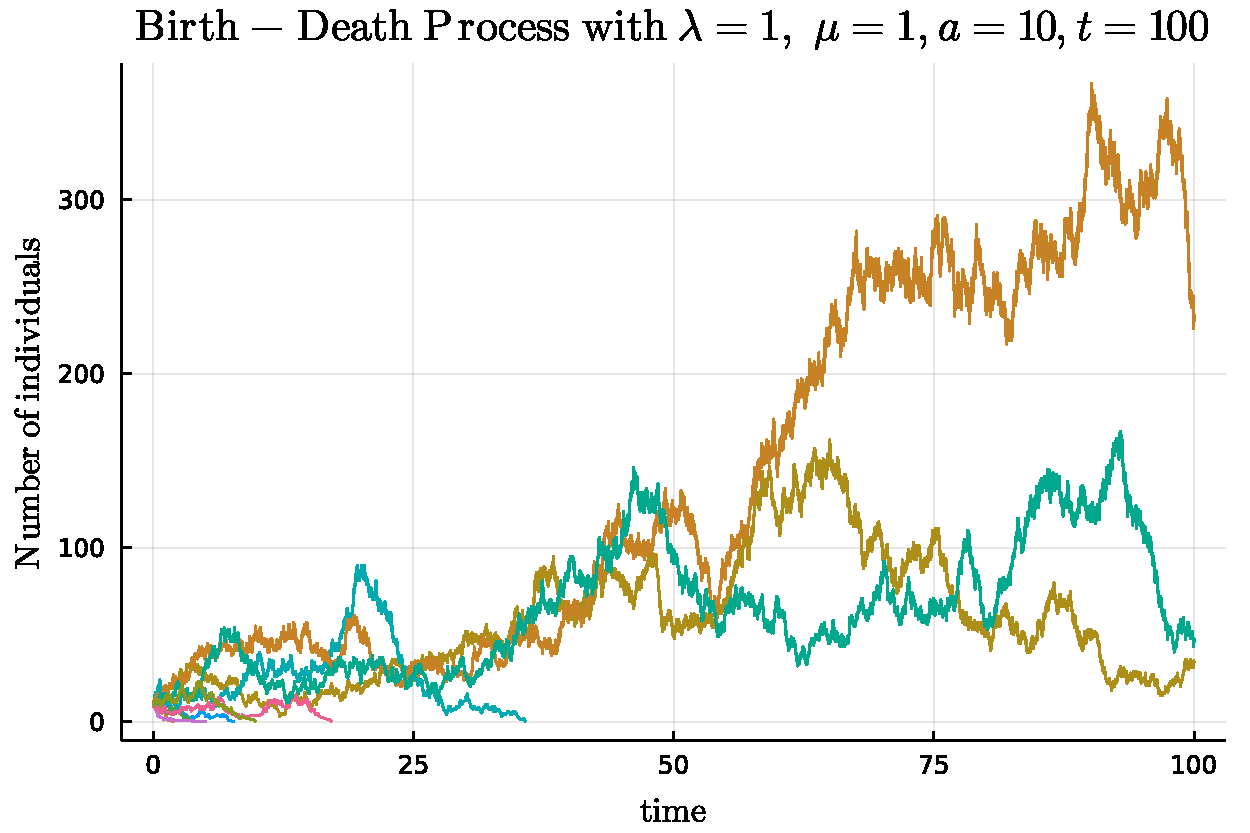
\includegraphics[scale=0.5]{pc.pdf}\\

\subsection{Part d}
Now, we set $\lambda=1.1$, $\mu=1$, $a=10$ and $t=50$ and 10 different runs on a log scale. Note that we have to remove the data points at which we have zero individuals in order to taking the log of zero. The following plot is produced. \\
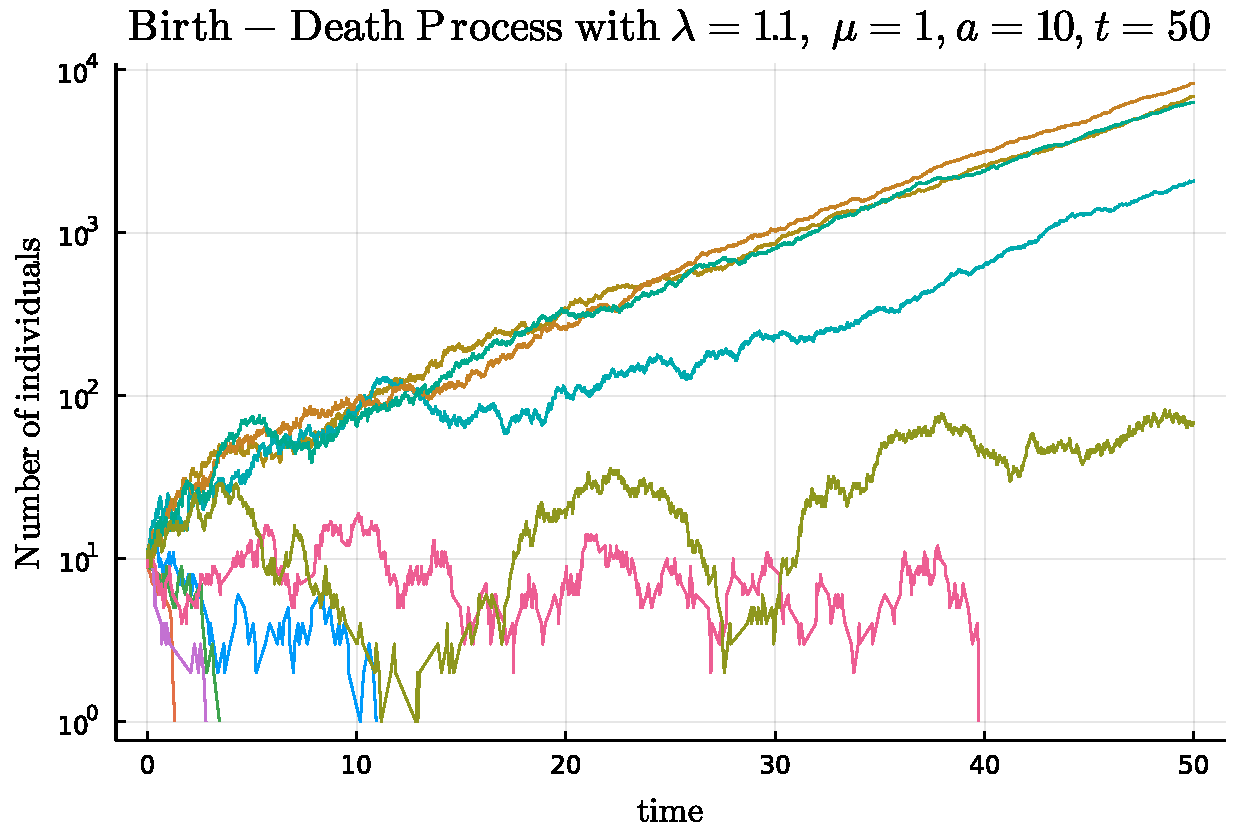
\includegraphics[scale=0.5]{pd.pdf}\\

\subsection{Part e}
In Julia, we write a function $\text{onerun}(t)$ which calls our simulation from before and returns the number of individuals present at time $t$. We also write a function $\text{simulation}(t,\text{numruns})$ which calls $\text{onerun}(t)$ numruns times to compute the average number of individuals present at time $t$.

\subsection{Part f}
We run the function simulation from part e first for $\lambda=\mu=1$, $a=10$, $t=0, 10,20,...,100$. In doing this, we use 50000 runs and obtain the following plot. \\
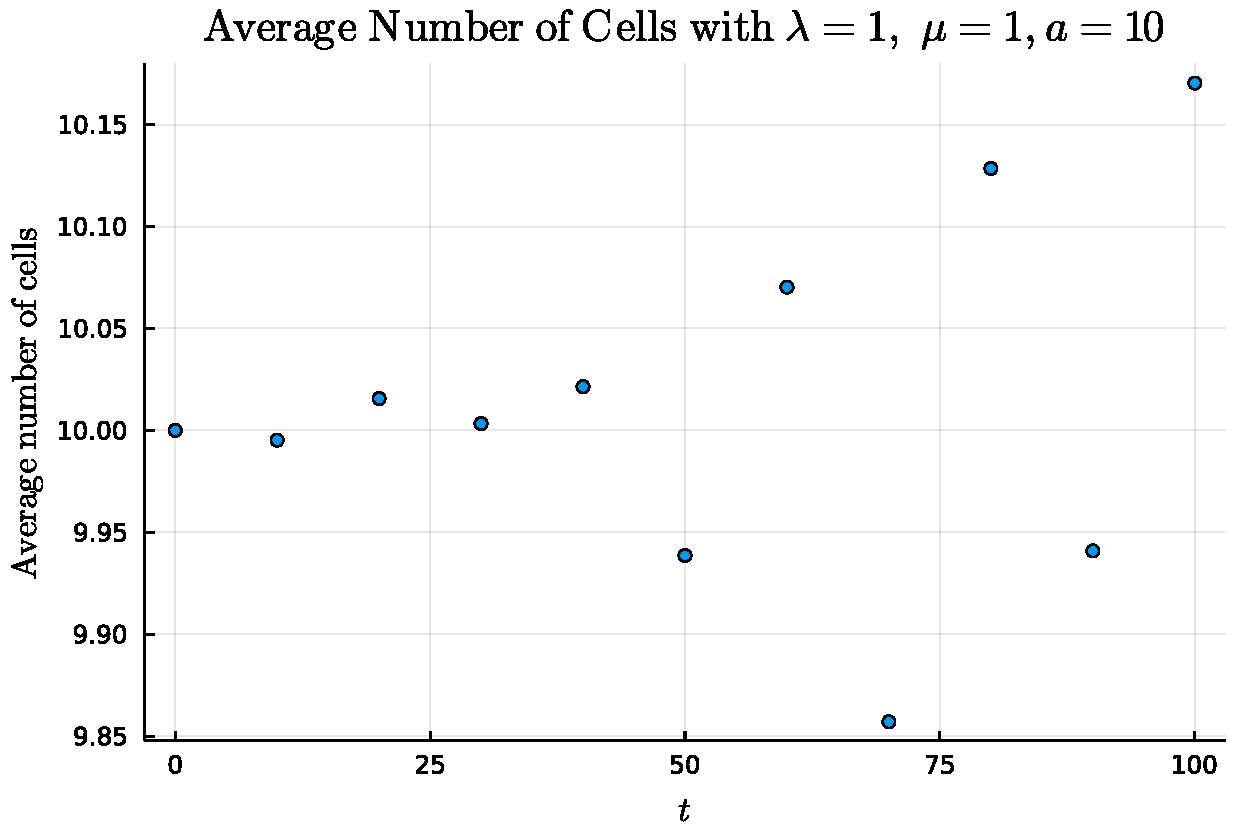
\includegraphics[scale=0.5]{pf1.pdf}\\
While this may look highly random, note that the scale of the y-axis is quite small relative to its values and that the result at each time is quite close to the population mean of 10 that we computed in problem 1. \\
Now, we run the function simulation from part e for $\lambda=1.1$, $\mu=1$, $a=10$, $t=0, 10,20,...,50$. Using only 500 runs this time, we obtain the following plot on a log scale. \\
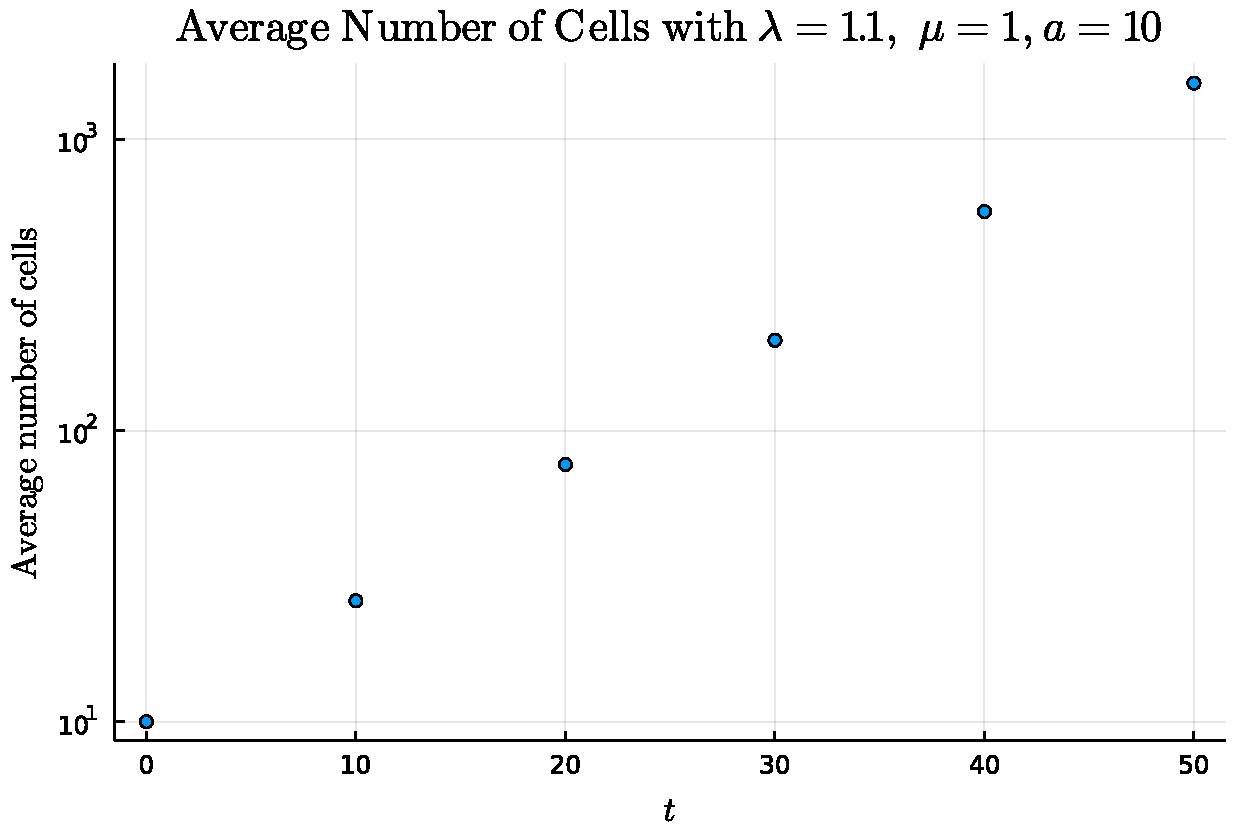
\includegraphics[scale=0.5]{pf2.pdf}\\
The points here clearly appear linear which implies that the average grows exponentially in $t$. 

\section{Appendix A}
The following is the Mathematica code used in problem 1. To compute the solution to the PDE in part b, we use
\begin{lstlisting}[language=Mathematica]
FullSimplify[
DSolve[{D[u[s, t], t] == \[Lambda] (s - 1)^2 D[u[s, t], s], 
	u[s, 0] == s^a}, u, {s, t}]]
\end{lstlisting}
and 
\begin{lstlisting}[language=Mathematica]
FullSimplify[(-1 + \[Lambda] (t + 
1/(\[Lambda] - s \[Lambda])))/(\[Lambda] (t + 
1/(\[Lambda] - s \[Lambda])))]
\end{lstlisting}
to get the form presented. For part c, we use the following commands
\begin{lstlisting}[language=Mathematica]
D[(-s + (-1 + s) t \[Lambda])/(-1 + (-1 + s) t \[Lambda]), {s, n}]
nderpb[s_, 
n_] := -((((t \[Lambda])/(1 + t (\[Lambda] - s \[Lambda])))^n n!)/(
t \[Lambda] (-1 + (-1 + s) t \[Lambda])))
FullSimplify[nderpb[0, n]]
\end{lstlisting}
to get the necessary derivatives. Finally, for part d, we use the commands
\begin{lstlisting}[language=Mathematica]
FullSimplify[nderpb[1, 1]]
FullSimplify[nderpb[1, 2]]
\end{lstlisting}

\section{Appendix B}
We use the following Julia code for problem 2. 
\jlinputlisting{Problem2.jl}

\end{document}
